% Created by tikzDevice version 0.12.6 on 2026-10-30 11:38:47
% !TEX encoding = UTF-8 Unicode
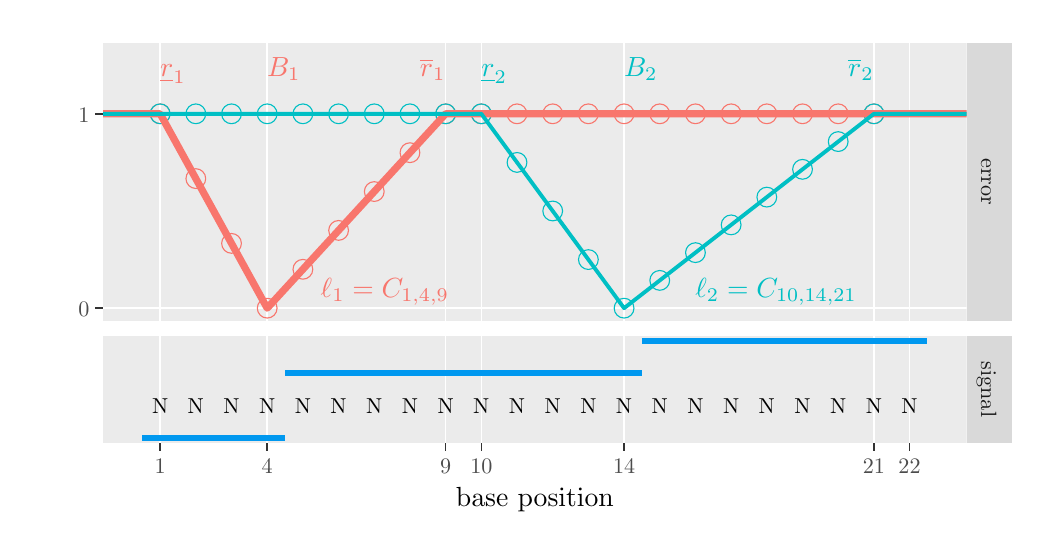
\begin{tikzpicture}[x=1pt,y=1pt]
\definecolor{fillColor}{RGB}{255,255,255}
\path[use as bounding box,fill=fillColor,fill opacity=0.00] (0,0) rectangle (361.35,180.67);
\begin{scope}
\path[clip] (  0.00,  0.00) rectangle (361.35,180.67);
\definecolor{drawColor}{RGB}{255,255,255}
\definecolor{fillColor}{RGB}{255,255,255}

\path[draw=drawColor,line width= 0.6pt,line join=round,line cap=round,fill=fillColor] (  0.00,  0.00) rectangle (361.35,180.68);
\end{scope}
\begin{scope}
\path[clip] ( 27.23, 74.75) rectangle (339.31,175.17);
\definecolor{fillColor}{gray}{0.92}

\path[fill=fillColor] ( 27.23, 74.75) rectangle (339.31,175.17);
\definecolor{drawColor}{RGB}{255,255,255}

\path[draw=drawColor,line width= 0.6pt,line join=round] ( 27.23,149.54) --
	(339.31,149.54);

\path[draw=drawColor,line width= 0.6pt,line join=round] ( 27.23, 79.31) --
	(339.31, 79.31);

\path[draw=drawColor,line width= 0.6pt,line join=round] ( 47.87, 74.75) --
	( 47.87,175.17);

\path[draw=drawColor,line width= 0.6pt,line join=round] ( 86.55, 74.75) --
	( 86.55,175.17);

\path[draw=drawColor,line width= 0.6pt,line join=round] (151.03, 74.75) --
	(151.03,175.17);

\path[draw=drawColor,line width= 0.6pt,line join=round] (163.93, 74.75) --
	(163.93,175.17);

\path[draw=drawColor,line width= 0.6pt,line join=round] (215.51, 74.75) --
	(215.51,175.17);

\path[draw=drawColor,line width= 0.6pt,line join=round] (305.78, 74.75) --
	(305.78,175.17);

\path[draw=drawColor,line width= 0.6pt,line join=round] (318.67, 74.75) --
	(318.67,175.17);
\definecolor{drawColor}{RGB}{248,118,109}

\node[text=drawColor,anchor=base west,inner sep=0pt, outer sep=0pt, scale=  1.00] at ( 47.87,163.04) {$\underline r_1$};

\node[text=drawColor,anchor=base west,inner sep=0pt, outer sep=0pt, scale=  1.00] at ( 86.55,163.04) {$B_1$};

\node[text=drawColor,anchor=base east,inner sep=0pt, outer sep=0pt, scale=  1.00] at (151.03,163.04) {$\overline r_1$};
\definecolor{drawColor}{RGB}{0,191,196}

\node[text=drawColor,anchor=base west,inner sep=0pt, outer sep=0pt, scale=  1.00] at (163.93,163.04) {$\underline r_2$};

\node[text=drawColor,anchor=base west,inner sep=0pt, outer sep=0pt, scale=  1.00] at (215.51,163.04) {$B_2$};

\node[text=drawColor,anchor=base east,inner sep=0pt, outer sep=0pt, scale=  1.00] at (305.78,163.04) {$\overline r_2$};
\definecolor{drawColor}{RGB}{248,118,109}

\path[draw=drawColor,line width= 0.4pt,line join=round,line cap=round] ( 47.87,149.54) circle (  3.57);

\path[draw=drawColor,line width= 0.4pt,line join=round,line cap=round] ( 60.76,126.13) circle (  3.57);

\path[draw=drawColor,line width= 0.4pt,line join=round,line cap=round] ( 73.66,102.72) circle (  3.57);

\path[draw=drawColor,line width= 0.4pt,line join=round,line cap=round] ( 86.55, 79.31) circle (  3.57);

\path[draw=drawColor,line width= 0.4pt,line join=round,line cap=round] ( 99.45, 93.36) circle (  3.57);

\path[draw=drawColor,line width= 0.4pt,line join=round,line cap=round] (112.35,107.41) circle (  3.57);

\path[draw=drawColor,line width= 0.4pt,line join=round,line cap=round] (125.24,121.45) circle (  3.57);

\path[draw=drawColor,line width= 0.4pt,line join=round,line cap=round] (138.14,135.50) circle (  3.57);

\path[draw=drawColor,line width= 0.4pt,line join=round,line cap=round] (151.03,149.54) circle (  3.57);

\path[draw=drawColor,line width= 0.4pt,line join=round,line cap=round] (163.93,149.54) circle (  3.57);

\path[draw=drawColor,line width= 0.4pt,line join=round,line cap=round] (176.82,149.54) circle (  3.57);

\path[draw=drawColor,line width= 0.4pt,line join=round,line cap=round] (189.72,149.54) circle (  3.57);

\path[draw=drawColor,line width= 0.4pt,line join=round,line cap=round] (202.61,149.54) circle (  3.57);

\path[draw=drawColor,line width= 0.4pt,line join=round,line cap=round] (215.51,149.54) circle (  3.57);

\path[draw=drawColor,line width= 0.4pt,line join=round,line cap=round] (228.40,149.54) circle (  3.57);

\path[draw=drawColor,line width= 0.4pt,line join=round,line cap=round] (241.30,149.54) circle (  3.57);

\path[draw=drawColor,line width= 0.4pt,line join=round,line cap=round] (254.20,149.54) circle (  3.57);

\path[draw=drawColor,line width= 0.4pt,line join=round,line cap=round] (267.09,149.54) circle (  3.57);

\path[draw=drawColor,line width= 0.4pt,line join=round,line cap=round] (279.99,149.54) circle (  3.57);

\path[draw=drawColor,line width= 0.4pt,line join=round,line cap=round] (292.88,149.54) circle (  3.57);

\path[draw=drawColor,line width= 0.4pt,line join=round,line cap=round] (305.78,149.54) circle (  3.57);
\definecolor{drawColor}{RGB}{0,191,196}

\path[draw=drawColor,line width= 0.4pt,line join=round,line cap=round] ( 47.87,149.54) circle (  3.57);

\path[draw=drawColor,line width= 0.4pt,line join=round,line cap=round] ( 60.76,149.54) circle (  3.57);

\path[draw=drawColor,line width= 0.4pt,line join=round,line cap=round] ( 73.66,149.54) circle (  3.57);

\path[draw=drawColor,line width= 0.4pt,line join=round,line cap=round] ( 86.55,149.54) circle (  3.57);

\path[draw=drawColor,line width= 0.4pt,line join=round,line cap=round] ( 99.45,149.54) circle (  3.57);

\path[draw=drawColor,line width= 0.4pt,line join=round,line cap=round] (112.35,149.54) circle (  3.57);

\path[draw=drawColor,line width= 0.4pt,line join=round,line cap=round] (125.24,149.54) circle (  3.57);

\path[draw=drawColor,line width= 0.4pt,line join=round,line cap=round] (138.14,149.54) circle (  3.57);

\path[draw=drawColor,line width= 0.4pt,line join=round,line cap=round] (151.03,149.54) circle (  3.57);

\path[draw=drawColor,line width= 0.4pt,line join=round,line cap=round] (163.93,149.54) circle (  3.57);

\path[draw=drawColor,line width= 0.4pt,line join=round,line cap=round] (176.82,131.98) circle (  3.57);

\path[draw=drawColor,line width= 0.4pt,line join=round,line cap=round] (189.72,114.43) circle (  3.57);

\path[draw=drawColor,line width= 0.4pt,line join=round,line cap=round] (202.61, 96.87) circle (  3.57);

\path[draw=drawColor,line width= 0.4pt,line join=round,line cap=round] (215.51, 79.31) circle (  3.57);

\path[draw=drawColor,line width= 0.4pt,line join=round,line cap=round] (228.40, 89.35) circle (  3.57);

\path[draw=drawColor,line width= 0.4pt,line join=round,line cap=round] (241.30, 99.38) circle (  3.57);

\path[draw=drawColor,line width= 0.4pt,line join=round,line cap=round] (254.20,109.41) circle (  3.57);

\path[draw=drawColor,line width= 0.4pt,line join=round,line cap=round] (267.09,119.44) circle (  3.57);

\path[draw=drawColor,line width= 0.4pt,line join=round,line cap=round] (279.99,129.48) circle (  3.57);

\path[draw=drawColor,line width= 0.4pt,line join=round,line cap=round] (292.88,139.51) circle (  3.57);

\path[draw=drawColor,line width= 0.4pt,line join=round,line cap=round] (305.78,149.54) circle (  3.57);
\definecolor{drawColor}{RGB}{248,118,109}

\path[draw=drawColor,line width= 2.6pt,line join=round] ( 27.23,149.54) --
	( 47.87,149.54) --
	( 86.55, 79.31) --
	(151.03,149.54) --
	(163.93,149.54) --
	(215.51,149.54) --
	(305.78,149.54) --
	(339.31,149.54);
\definecolor{drawColor}{RGB}{0,191,196}

\path[draw=drawColor,line width= 1.4pt,line join=round] ( 27.23,149.54) --
	( 47.87,149.54) --
	( 86.55,149.54) --
	(151.03,149.54) --
	(163.93,149.54) --
	(215.51, 79.31) --
	(305.78,149.54) --
	(339.31,149.54);
\definecolor{drawColor}{RGB}{248,118,109}

\node[text=drawColor,anchor=base west,inner sep=0pt, outer sep=0pt, scale=  1.00] at (105.90, 83.10) {$\ell_1 = C_{1,4,9}$};
\definecolor{drawColor}{RGB}{0,191,196}

\node[text=drawColor,anchor=base west,inner sep=0pt, outer sep=0pt, scale=  1.00] at (241.30, 83.10) {$\ell_2 = C_{10,14,21}$};
\end{scope}
\begin{scope}
\path[clip] ( 27.23, 30.62) rectangle (339.31, 69.25);
\definecolor{fillColor}{gray}{0.92}

\path[fill=fillColor] ( 27.23, 30.62) rectangle (339.31, 69.25);
\definecolor{drawColor}{RGB}{255,255,255}

\path[draw=drawColor,line width= 0.6pt,line join=round] ( 47.87, 30.62) --
	( 47.87, 69.25);

\path[draw=drawColor,line width= 0.6pt,line join=round] ( 86.55, 30.62) --
	( 86.55, 69.25);

\path[draw=drawColor,line width= 0.6pt,line join=round] (151.03, 30.62) --
	(151.03, 69.25);

\path[draw=drawColor,line width= 0.6pt,line join=round] (163.93, 30.62) --
	(163.93, 69.25);

\path[draw=drawColor,line width= 0.6pt,line join=round] (215.51, 30.62) --
	(215.51, 69.25);

\path[draw=drawColor,line width= 0.6pt,line join=round] (305.78, 30.62) --
	(305.78, 69.25);

\path[draw=drawColor,line width= 0.6pt,line join=round] (318.67, 30.62) --
	(318.67, 69.25);
\definecolor{drawColor}{RGB}{0,152,239}

\path[draw=drawColor,line width= 2.3pt,line join=round] ( 41.42, 32.38) -- ( 93.00, 32.38);

\path[draw=drawColor,line width= 2.3pt,line join=round] ( 93.00, 55.79) -- (221.96, 55.79);

\path[draw=drawColor,line width= 2.3pt,line join=round] (221.96, 67.49) -- (325.12, 67.49);
\definecolor{drawColor}{RGB}{0,0,0}

\node[text=drawColor,anchor=base,inner sep=0pt, outer sep=0pt, scale=  0.78] at ( 47.87, 41.16) {N};

\node[text=drawColor,anchor=base,inner sep=0pt, outer sep=0pt, scale=  0.78] at ( 60.76, 41.16) {N};

\node[text=drawColor,anchor=base,inner sep=0pt, outer sep=0pt, scale=  0.78] at ( 73.66, 41.16) {N};

\node[text=drawColor,anchor=base,inner sep=0pt, outer sep=0pt, scale=  0.78] at ( 86.55, 41.16) {N};

\node[text=drawColor,anchor=base,inner sep=0pt, outer sep=0pt, scale=  0.78] at ( 99.45, 41.16) {N};

\node[text=drawColor,anchor=base,inner sep=0pt, outer sep=0pt, scale=  0.78] at (112.35, 41.16) {N};

\node[text=drawColor,anchor=base,inner sep=0pt, outer sep=0pt, scale=  0.78] at (125.24, 41.16) {N};

\node[text=drawColor,anchor=base,inner sep=0pt, outer sep=0pt, scale=  0.78] at (138.14, 41.16) {N};

\node[text=drawColor,anchor=base,inner sep=0pt, outer sep=0pt, scale=  0.78] at (151.03, 41.16) {N};

\node[text=drawColor,anchor=base,inner sep=0pt, outer sep=0pt, scale=  0.78] at (163.93, 41.16) {N};

\node[text=drawColor,anchor=base,inner sep=0pt, outer sep=0pt, scale=  0.78] at (176.82, 41.16) {N};

\node[text=drawColor,anchor=base,inner sep=0pt, outer sep=0pt, scale=  0.78] at (189.72, 41.16) {N};

\node[text=drawColor,anchor=base,inner sep=0pt, outer sep=0pt, scale=  0.78] at (202.61, 41.16) {N};

\node[text=drawColor,anchor=base,inner sep=0pt, outer sep=0pt, scale=  0.78] at (215.51, 41.16) {N};

\node[text=drawColor,anchor=base,inner sep=0pt, outer sep=0pt, scale=  0.78] at (228.40, 41.16) {N};

\node[text=drawColor,anchor=base,inner sep=0pt, outer sep=0pt, scale=  0.78] at (241.30, 41.16) {N};

\node[text=drawColor,anchor=base,inner sep=0pt, outer sep=0pt, scale=  0.78] at (254.20, 41.16) {N};

\node[text=drawColor,anchor=base,inner sep=0pt, outer sep=0pt, scale=  0.78] at (267.09, 41.16) {N};

\node[text=drawColor,anchor=base,inner sep=0pt, outer sep=0pt, scale=  0.78] at (279.99, 41.16) {N};

\node[text=drawColor,anchor=base,inner sep=0pt, outer sep=0pt, scale=  0.78] at (292.88, 41.16) {N};

\node[text=drawColor,anchor=base,inner sep=0pt, outer sep=0pt, scale=  0.78] at (305.78, 41.16) {N};

\node[text=drawColor,anchor=base,inner sep=0pt, outer sep=0pt, scale=  0.78] at (318.67, 41.16) {N};
\end{scope}
\begin{scope}
\path[clip] (339.31, 74.75) rectangle (355.85,175.17);
\definecolor{fillColor}{gray}{0.85}

\path[fill=fillColor] (339.31, 74.75) rectangle (355.85,175.17);
\definecolor{drawColor}{gray}{0.10}

\node[text=drawColor,rotate=-90.00,anchor=base,inner sep=0pt, outer sep=0pt, scale=  0.80] at (344.56,124.96) {error};
\end{scope}
\begin{scope}
\path[clip] (339.31, 30.62) rectangle (355.85, 69.25);
\definecolor{fillColor}{gray}{0.85}

\path[fill=fillColor] (339.31, 30.62) rectangle (355.85, 69.25);
\definecolor{drawColor}{gray}{0.10}

\node[text=drawColor,rotate=-90.00,anchor=base,inner sep=0pt, outer sep=0pt, scale=  0.80] at (344.56, 49.94) {signal};
\end{scope}
\begin{scope}
\path[clip] (  0.00,  0.00) rectangle (361.35,180.67);
\definecolor{drawColor}{gray}{0.20}

\path[draw=drawColor,line width= 0.6pt,line join=round] ( 47.87, 27.87) --
	( 47.87, 30.62);

\path[draw=drawColor,line width= 0.6pt,line join=round] ( 86.55, 27.87) --
	( 86.55, 30.62);

\path[draw=drawColor,line width= 0.6pt,line join=round] (151.03, 27.87) --
	(151.03, 30.62);

\path[draw=drawColor,line width= 0.6pt,line join=round] (163.93, 27.87) --
	(163.93, 30.62);

\path[draw=drawColor,line width= 0.6pt,line join=round] (215.51, 27.87) --
	(215.51, 30.62);

\path[draw=drawColor,line width= 0.6pt,line join=round] (305.78, 27.87) --
	(305.78, 30.62);

\path[draw=drawColor,line width= 0.6pt,line join=round] (318.67, 27.87) --
	(318.67, 30.62);
\end{scope}
\begin{scope}
\path[clip] (  0.00,  0.00) rectangle (361.35,180.67);
\definecolor{drawColor}{gray}{0.30}

\node[text=drawColor,anchor=base,inner sep=0pt, outer sep=0pt, scale=  0.80] at ( 47.87, 19.64) {1};

\node[text=drawColor,anchor=base,inner sep=0pt, outer sep=0pt, scale=  0.80] at ( 86.55, 19.64) {4};

\node[text=drawColor,anchor=base,inner sep=0pt, outer sep=0pt, scale=  0.80] at (151.03, 19.64) {9};

\node[text=drawColor,anchor=base,inner sep=0pt, outer sep=0pt, scale=  0.80] at (163.93, 19.64) {10};

\node[text=drawColor,anchor=base,inner sep=0pt, outer sep=0pt, scale=  0.80] at (215.51, 19.64) {14};

\node[text=drawColor,anchor=base,inner sep=0pt, outer sep=0pt, scale=  0.80] at (305.78, 19.64) {21};

\node[text=drawColor,anchor=base,inner sep=0pt, outer sep=0pt, scale=  0.80] at (318.67, 19.64) {22};
\end{scope}
\begin{scope}
\path[clip] (  0.00,  0.00) rectangle (361.35,180.67);
\definecolor{drawColor}{gray}{0.30}

\node[text=drawColor,anchor=base east,inner sep=0pt, outer sep=0pt, scale=  0.80] at ( 22.28,146.53) {1};

\node[text=drawColor,anchor=base east,inner sep=0pt, outer sep=0pt, scale=  0.80] at ( 22.28, 76.30) {0};
\end{scope}
\begin{scope}
\path[clip] (  0.00,  0.00) rectangle (361.35,180.67);
\definecolor{drawColor}{gray}{0.20}

\path[draw=drawColor,line width= 0.6pt,line join=round] ( 24.48,149.54) --
	( 27.23,149.54);

\path[draw=drawColor,line width= 0.6pt,line join=round] ( 24.48, 79.31) --
	( 27.23, 79.31);
\end{scope}
\begin{scope}
\path[clip] (  0.00,  0.00) rectangle (361.35,180.67);
\definecolor{drawColor}{RGB}{0,0,0}

\node[text=drawColor,anchor=base,inner sep=0pt, outer sep=0pt, scale=  1.00] at (183.27,  7.64) {base position};
\end{scope}
\end{tikzpicture}
